\documentclass[12pt]{article}

\usepackage[utf8]{inputenc}
\usepackage[danish]{babel}
\usepackage{graphicx}
\usepackage{latexsym, amsfonts, amssymb, amsthm, amsmath, siunitx, pgfplots}
\usepackage[hidelinks]{hyperref}

\sisetup{exponent-product = \cdot,
  output-decimal-marker = {,}}

%Giles Castelles incfig
\usepackage{import}
\usepackage{xifthen}
\usepackage{pdfpages}
\usepackage{transparent}

\newcommand{\incfig}[2][1]{%
    \def\svgwidth{#1\columnwidth}
    \import{../figures/}{#2.pdf_tex}
}

\pdfsuppresswarningpagegroup=1

\setlength{\parindent}{0in}
\setlength{\oddsidemargin}{0in}
\setlength{\textwidth}{6.5in}
\setlength{\textheight}{8.8in}
\setlength{\topmargin}{0in}
\setlength{\headheight}{18pt}

\pgfplotsset{compat=newest}

\pgfplotsset{every axis/.append style={
  axis x line=middle,    % put the x axis in the middle
  axis y line=middle,    % put the y axis in the middle
  axis line style={<->,color=black}, % arrows on the axis
}}

\title{Opgaver til forelæsning 8}
\author{Noah Rahbek Bigum Hansen}
\date{8. Oktober 2024}

\begin{document}

\maketitle

\section*{Opg. 5.6}
A large wrecking ball is held in place by two light steel cables (\textbf{\autoref{fig:E5_6}}). If the mass $m$ of the wrecking ball is \qty{3620}{kg}, what are

\begin{figure} [ht]
  \centering
  \caption{}
  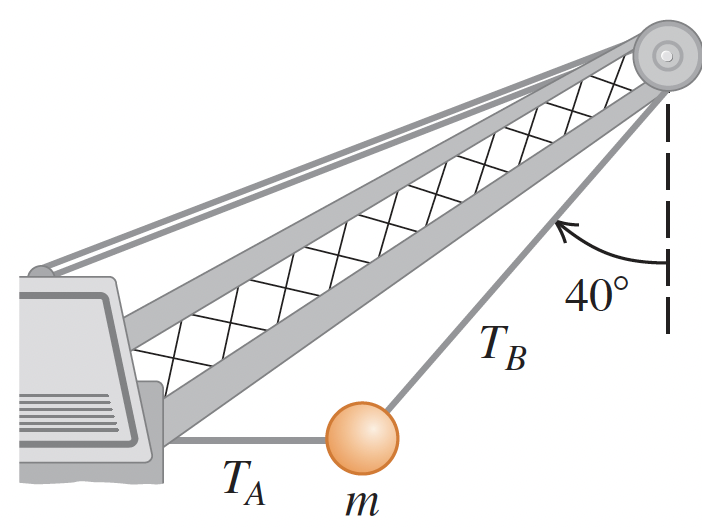
\includegraphics[width=0.5\linewidth]{../figures/E5_6.png}
  \label{fig:E5_6}
\end{figure}

\subsection*{(a)}
The tension $T_B$ in the cable that makes the angle of \ang{40} with the vertical and
\bigbreak
Al boldens vægt må blive holdt af kablet der har en vinkel på \ang{40} til vertikal. Altså må spændingen i dette reb, $T_B$, være netop så stor at dens lodrette komponent tilsvarer boldens vægt. Boldens vægt findes først vha. Newtons 2. lov. Her får vi at
 \[
F = ma \implies T_{B_y} = m_{ball}\cdot g = \qty{3620}{kg}\cdot g = \qty{35,512}{kN}
.\] 
Dernæst kan spændingen i rebet, $T_B$, findes vha. trigonometri. Her får vi at
 \[
T_B = \frac{T_{B_y}}{\cos(\alpha)} \implies T_B = \frac{\qty{35,512}{kN}}{\cos( \ang{40})} = \qty{46,357}{kN}
.\] 
Altså er spændingen i rebet, $T_B = \qty{46}{kN}$

\subsection*{(b)}
The tension $T_A$ in the horizontal cable?
\bigbreak
Idet der er statisk ligevægt må det gælde at $T_A + T_{B_x} = 0$. For at finde $T_{B_x}$ kan trigonometri benyttes. Her får vi at
\[
T_{B_x} = T_B \cdot \sin(\alpha) \implies T_{B_x} = \qty{46,358}{kN} \cdot \sin( \ang{40}) = \qty{29,798}{kN}
.\] 
Altså er spændingen i rebet \qty{29}{kN}.


\section*{Opg. 5.7} 
Find the tension in each cord in (\textbf{\autoref{fig:E5_7}}) if the weight of the suspended object is $w$.

\begin{figure} [ht]
  \centering
  \caption{}
  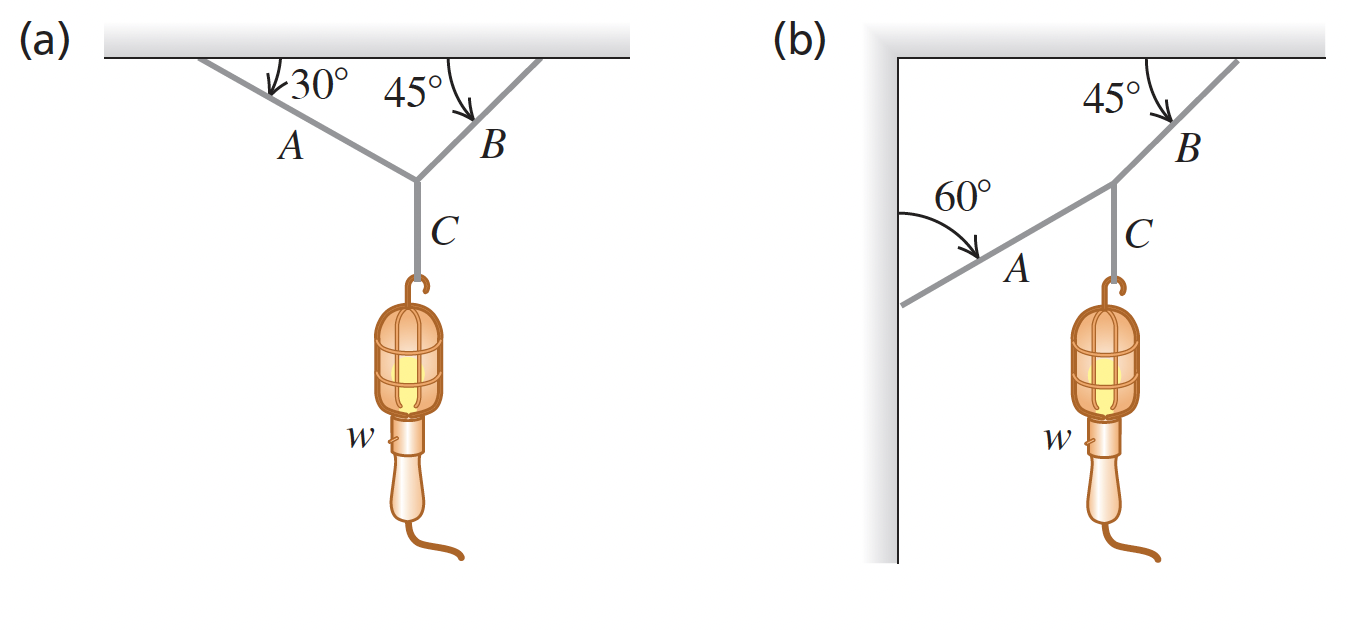
\includegraphics[width=0.75\linewidth]{../figures/E5_7.png}
  \label{fig:E5_7}
\end{figure}

\subsection*{(a)}
Med samme argument som ovenfor må det gælde at de to rebs $x$-komposanter udligner hinanden. Altså har vi at
 \[
A_x =- B_x
.\] 
$x$-komposanterne må være givet ved
 \[
\cos( \ang{30}) \cdot A = \cos( \ang{45}) \cdot B \implies A = \frac{\cos(\ang{45})}{\cos(\ang{30}}B
.\] 
$y$-komposanterne må netop opveje massen således at
 \[
A_y + B_y = w
.\]
y-komposanterne må desuden kunne skrives som
\[
\sin(\ang{30})\cdot A + \sin(\ang{45})B = w
.\] 
Heri kan indsættes vores udtryk for A, så vi får at
\[
  \frac{\sin(\ang{30})\cdot \cos(\ang{45})}{\cos(\ang{30})}B + \sin(\ang{45})B = w \implies B = \frac{w}{\frac{\sin(\ang{30})\cdot \cos(\ang{45})}{\cos(\ang{30})}+\sin(\ang{45})} = \num{0,897}w
.\]
Og spændingen i rebet A kan da findes vha. ligningen
\[
  A = \frac{\cos(\ang{45})}{\cos(\ang{30})}\cdot B = \frac{\cos(\ang{45})}{\cos(\ang{30})} \cdot \num{0,897}w = \num{0,732}w
.\] 


\subsection*{(b)}
Opgave B ville skulle løses på samme måde, dog skal man her være opmærksom på at vinklen til A er $\ang{180}-\ang{60}$ og ikke blot de oplyste \ang{60}.

\section*{Opg. 5.8}
In (\textbf{\autoref{fig:E5_8}}) the weight $w$ is  \qty{60.0}{N}.

\begin{figure} [ht]
  \centering
  \caption{}
  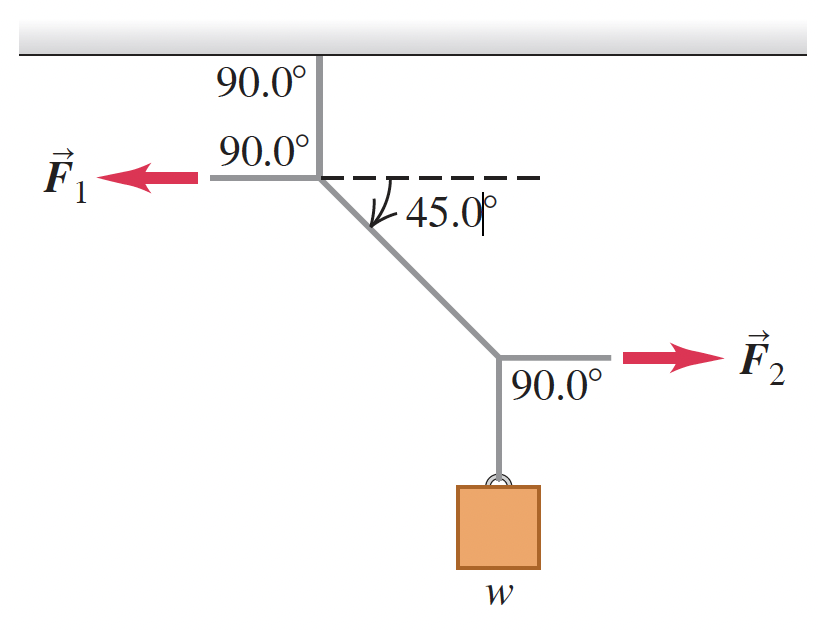
\includegraphics[width=0.5\linewidth]{../figures/E5_8.png}
  \label{fig:E5_8}
\end{figure}

\subsection*{(a)}
What is the tension in the diagonal string?
\bigbreak
Den lodrette komponent af spændingen i det diagonale reb må netop tilsvare vægten $w$. Altså har vi at
 \[
T_y = w \implies \sin(\ang{45})\cdot T = w \implies T = \frac{w}{\sin(\ang{45})} = \frac{\qty{60,0}{N}}{\sin(\ang{45})} = \qty{84,9}{N}
.\] 

\subsection*{(b)}
Find the magnitudes of the horizontal forces $\Vec{F_1}$ and $\Vec{F_2}$ that must be applied to hold the system in the position shown.
\bigbreak
Idet der er statisk ligevægt må de to kræfter, $\Vec{F_1}$ og $\Vec{F_2}$, være lige store idet de er modsatrettede. Den samlede vandrette spænding i rebet må i øvrigt tilsvare disse kræfter. Altså har vi at
\[
T_x = |\Vec{F_1}| = |\Vec{F_2}|
.\] 
Den vandrette spænding i rebet kan findes vha. trigonometri så vi får at
\[
T_x = \cos(\ang{45})\cdot T = \cos(\ang{45})\cdot \qty{84,9}{N} = \qty{60,0}{N} 
.\] 
Altså må den vandrette spænding i rebet netop tilsvare vægten  $w$. Dette giver god mening da det burde forventes at en ens kraft i  $x$- og  $y$-retningen medfører en vinkel på  \ang{45}.

\section*{Opg. 5.15}
\textbf{Atwood's machine.} A \qty{15.0}{kg} load of bricks hangs from one end of a rope that passes over a small, frictionless pulley.
A \qty{28.0}{kg} counterweight is suspended from the other end of the rope (\textbf{\autoref{fig:E5_15}}). The system is released from rest.
\begin{figure} [ht]
  \centering
  \caption{}
  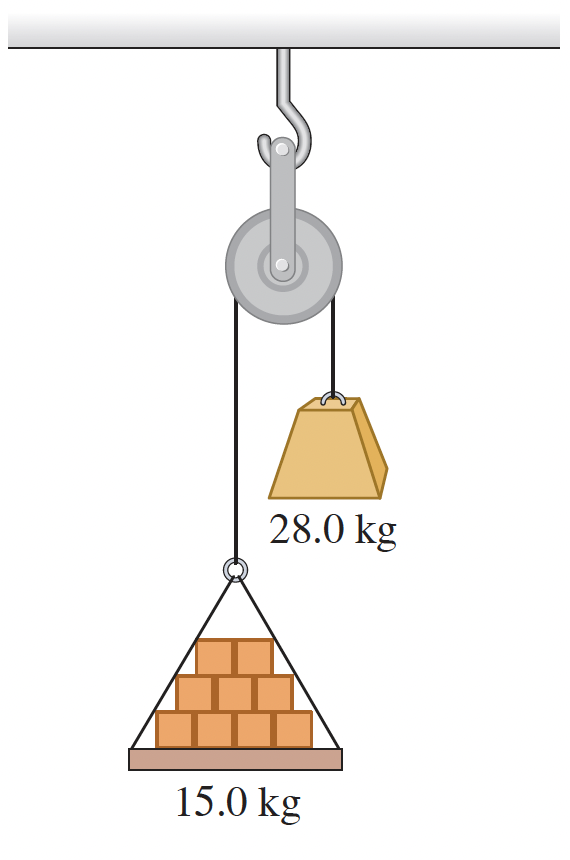
\includegraphics[width=0.25\linewidth]{../figures/E5_15.png}
  \label{fig:E5_15}
\end{figure}

\subsection*{(a)}
Draw two free-body diagrams, one for the load of bricks and one for the counterweight.
\bigbreak
De to fritlegemediagrammer er anført som hhv. (\textbf{\autoref{fig:E5_15a}}) og (\textbf{\autoref{fig:E5_15a1}}) 

\begin{figure}[ht]
  \begin{minipage}[c]{0.4\linewidth}
    \centering
    \incfig[1]{E5_15a}
    \caption{Fritlegemediagram for murstenene}
    \label{fig:E5_15a}
  \end{minipage}\hfill
  \begin{minipage}[c]{0.4\linewidth}
    \centering
    \incfig[1]{E5_15a1}
    \caption{Fritlegemediagram for modvægten}
    \label{fig:E5_15a1}
  \end{minipage}
\end{figure}  


\subsection*{(b)}
What is the magnitude of the upward acceleration of the load of bricks?
\bigbreak
Den samlede kraft i rebet må være givet ved differensen mellem de to vægte. Altså har vi at
\[
\Vec{F} = w_{cw} - w_{b} = (\qty{28,0}{kg} - \qty{15,0}{kg})\cdot g  = \qty{13,0}{kg} \cdot  g = \qty{127,4}{N}
.\]
Den samlede acceleration må således kunne findes ved Newtons 2. lov. Altså har vi at
\[
  a = \frac{\Vec{F}}{m_{total}} = \frac{\qty{127,4}{N}}{\qty{43.0}{kg}} = \qty{2,96}{\frac{m}{s^2}}
.\] 

\subsection*{(c)}
What is the tension in the rope while the load is moving? How does the tension compare to the weight of the load of bricks? To the weight of the counterweight?
\bigbreak
Spændingen i rebet er fundet i sidste opgave til \qty{127,4}{N} hvilket er differensen mellem de to vægte.  


\section*{Opg. 5.45}
small remote-controlled car with mass \qty{1.60}{kg} moves at a constant speed of $v = \qty{12.0}{\frac{m}{s}}$ in a track formed by a vertical circle inside a hollow metal cylinder that has a radius of  \qty{5.00}{m} (\textbf{\autoref{fig:E5_45}}). What is the magnitude of the normal force exerted on the car by the walls of the cylinder at

\begin{figure} [ht]
  \centering
  \caption{}
  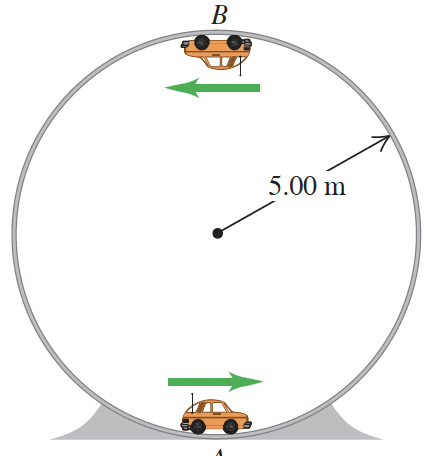
\includegraphics[width=0.25\linewidth]{../figures/E5_45.png}
  \label{fig:E5_45}
\end{figure}

\subsection*{(a)}
point $A$ (bottom of the track) and
\bigbreak
Den radiale acceleration som bilen oplever qua sin cirkelbevægelse er givet ved
\[
  a_{rad} = \frac{v^2}{R} \implies a_{rad} = \frac{(\qty{12,0}{\frac{m}{s}})^2}{\qty{5,00}{m}} = \qty{28,8}{\frac{m}{s^2}} 
.\] 
I bunden af banen må tyngdekraften pege i samme retning som den radiale acceleration og dermed må den samlede acceleration i bunden være
\[
a_{bund} = a_{rad} + g = \qty{28,8}{\frac{m}{s^2}} + \qty{9,81}{\frac{m}{s^2}} = \qty{38,6}{\frac{m}{s^2}}
.\] 

\subsection*{(b)}
point $B$ (top of the track)?
\bigbreak
I toppen af ringen må tyngdekraften pege modsat den radiale acceleration og derfor må den samlede acceleration i toppen være
\[
a_{top} = a_{rad} - g = \qty{28,8}{\frac{m}{s^2}} - \qty{9,81}{\frac{m}{s^2}} = \qty{19,0}{\frac{m}{s^2}}
.\] 
  

\section*{Opg. 5.53}
\textbf{Rotating Space Stations.}
One problem for humans living in outer space is that they are apparently weightless.
One way around this problem is to design a space station that spins about its center at a constant rate. 
This creates “artificial gravity” at the outside rim of the station.


\subsection*{(a)}
If the diameter of the space station is \qty{800}{m}, how many revolutions per minute are needed for the “artificial gravity” acceleration to be \qty{9.80}{m/s^2}?  
\bigbreak
Den kunstige tyngdekraft må tilsvare den radiale acceleration således har vi at $a_{rad} = \qty{9,80}{\frac{m}{s^2}}$. Al kendt info sættes ind i formlen for radial acceleration så vi får at:
\[
v = \sqrt{a_{rad}\cdot R} \implies v = \sqrt{\qty{9,80}{\frac{m}{s^2}}\cdot \qty{400}{m}} = \qty{62,60}{\frac{m}{s}}
.\] 
Antallet af RPM kan da findes som
\[
  \unit{RPM} = \frac{v}{2\pi\cdot R} \implies \unit{RPM} = \frac{\qty{62,60}{\frac{m}{s^2}}}{2\pi\cdot \qty{400}{m}} = \qty{1,49}{RPM}
.\] 


\subsection*{(b)}
If the space station is a waiting area for travelers going to Mars, it might be desirable to simulate the acceleration due to gravity on the Martian surface (\qty{3.70}{m/s^2}). 
How many revolutions per minute are needed in this case?
\bigbreak
Med samme fremgangsmåde som ovenfor har vi at:
\[
v = \sqrt{\qty{3,70}{\frac{m}{s^2}}\cdot \qty{400}{m}}  = \qty{38,47}{\frac{m}{s}}
.\] 
Og altså at
\[
  \unit{RPM} = \frac{\qty{38,47}{\frac{m}{s}}}{2\pi\cdot \qty{400}{m}} = \qty{0,918}{RPM}
.\] 

\section*{Opg. 5.101}
A racetrack curve has radius \qty{90.0}{m} and is banked at an angle of \ang{18.0}.
The coefficient of static friction between the tires and the roadway is \num{0.400}.
A race car with mass \qty{1200}{kg} rounds the curve with the maximum speed to avoid skidding.

\begin{figure}[ht]
  \centering
  \incfig[0.8]{E5_101}
  \caption{}
  \label{fig:E5_101}
\end{figure}

\subsection*{(a)}
As the car rounds the curve, what is the normal force exerted on it by the road?
\bigbreak
Som kan ses på (\textbf{\autoref{fig:E5_101}}) er der konstrueret et fritlegemediagram for situationen. Heraf kan også ses, at den samlede normalkraft på bilen må svare til summen af de lodrette komponenter ift. vejen af centripetalkraften og tyngdekraften på bilen. Heraf kan også ses at den lodrette komponent af tyngdekraften må være givet ved
\[
  \Vec{F_{t_y}} = \cos(\ang{18})\cdot m\cdot g \implies \Vec{F_{t_y}} = \cos(\ang{18})\cdot \qty{1200}{kg}\cdot \qty{9,81}{\frac{m}{s^2}} = \qty{11,1}{kN}
,\] 
Og den lodrette komponent af centripetalkraften må være
\[
\Vec{F_{c_y}} = \sin(\ang{18})\cdot m\cdot a_{rad} = 
.\] 

\subsection*{(b)}
What is the cars radial acceleration?


\subsection*{(c)}
What is the cars speed?

  

\end{document}
